\documentclass[../main.tex]{subfiles}
\begin{document}
\part*{Project Background}
Image recognition, also known as computer vision, is a field of study in artificial intelligence that involves training computer systems to identify, interpret, and understand images or visual data. It involves developing algorithms and models that can recognize patterns, objects, and features within an image or video.

\begin{figure}[h!]
\centering
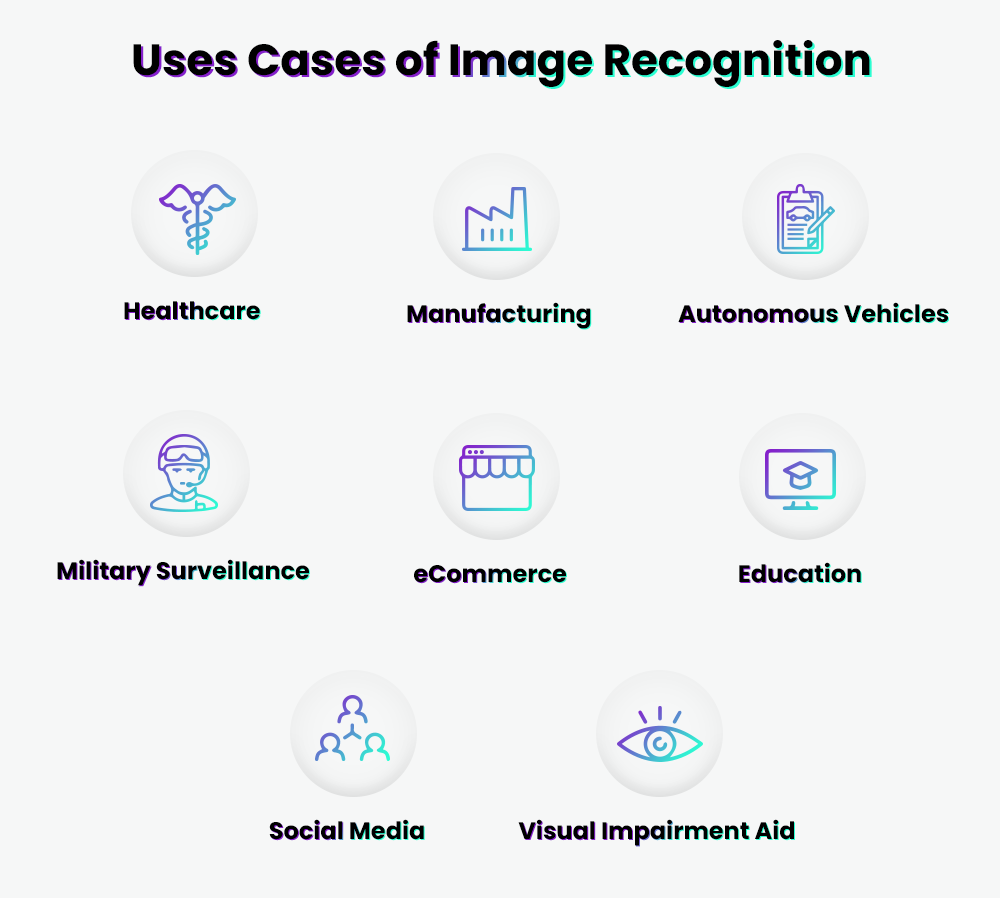
\includegraphics[scale=0.3]{images/image_rec_uses.png}
\caption{Some use-cases of Image Recognition.\citet{im}}
\label{fig:im_uses}
\end{figure}

Image recognition has a wide range of applications across various industries such as healthcare, automotive, retail, security, and entertainment. Some examples include:
\begin{itemize}
    \item \textbf{Healthcare}: image recognition technology can be used for medical imaging analysis, disease diagnosis, and drug discovery.
    \item \textbf{Automotive}: image recognition can be used for autonomous driving, traffic monitoring, and vehicle safety features.
    \item \textbf{Retail}: image recognition can be used for product recognition, inventory management, and customer behavior analysis.
    \item \textbf{Security}: image recognition can be used for facial recognition, object detection, and surveillance monitoring.
    \item \textbf{Entertainment}: image recognition can be used for augmented reality, virtual reality, and gaming.
\end{itemize}

\textbf{IaaS} (Infrastructure as a Service) is a cloud computing model in which cloud service providers offer virtualized computing resources such as servers, storage, and networking to users on a pay-per-use basis. IaaS allows users to scale up or down their computing resources as needed, without having to invest in their own infrastructure. Examples of IaaS providers include Amazon Web Services, Microsoft Azure, and Google Cloud Platform.

IaaS services have a wide range of applications across various industries, such as:
\begin{itemize}
    \item \textbf{Web hosting}: IaaS providers can host websites and web applications in the cloud, providing scalable and reliable infrastructure.
    \item \textbf{Big data}: IaaS providers can provide the computing resources needed to process and analyze large volumes of data.
    \item \textbf{Disaster recovery}: IaaS providers can provide backup and recovery solutions in the event of a disaster or outage.
    \item \textbf{DevOps}: IaaS providers can provide the infrastructure needed for software development and testing.
    \item \textbf{Machine learning}: IaaS providers can provide the computing resources needed to train and run machine learning models.
\end{itemize}





\end{document}

\clearpage